\subsection{Model}

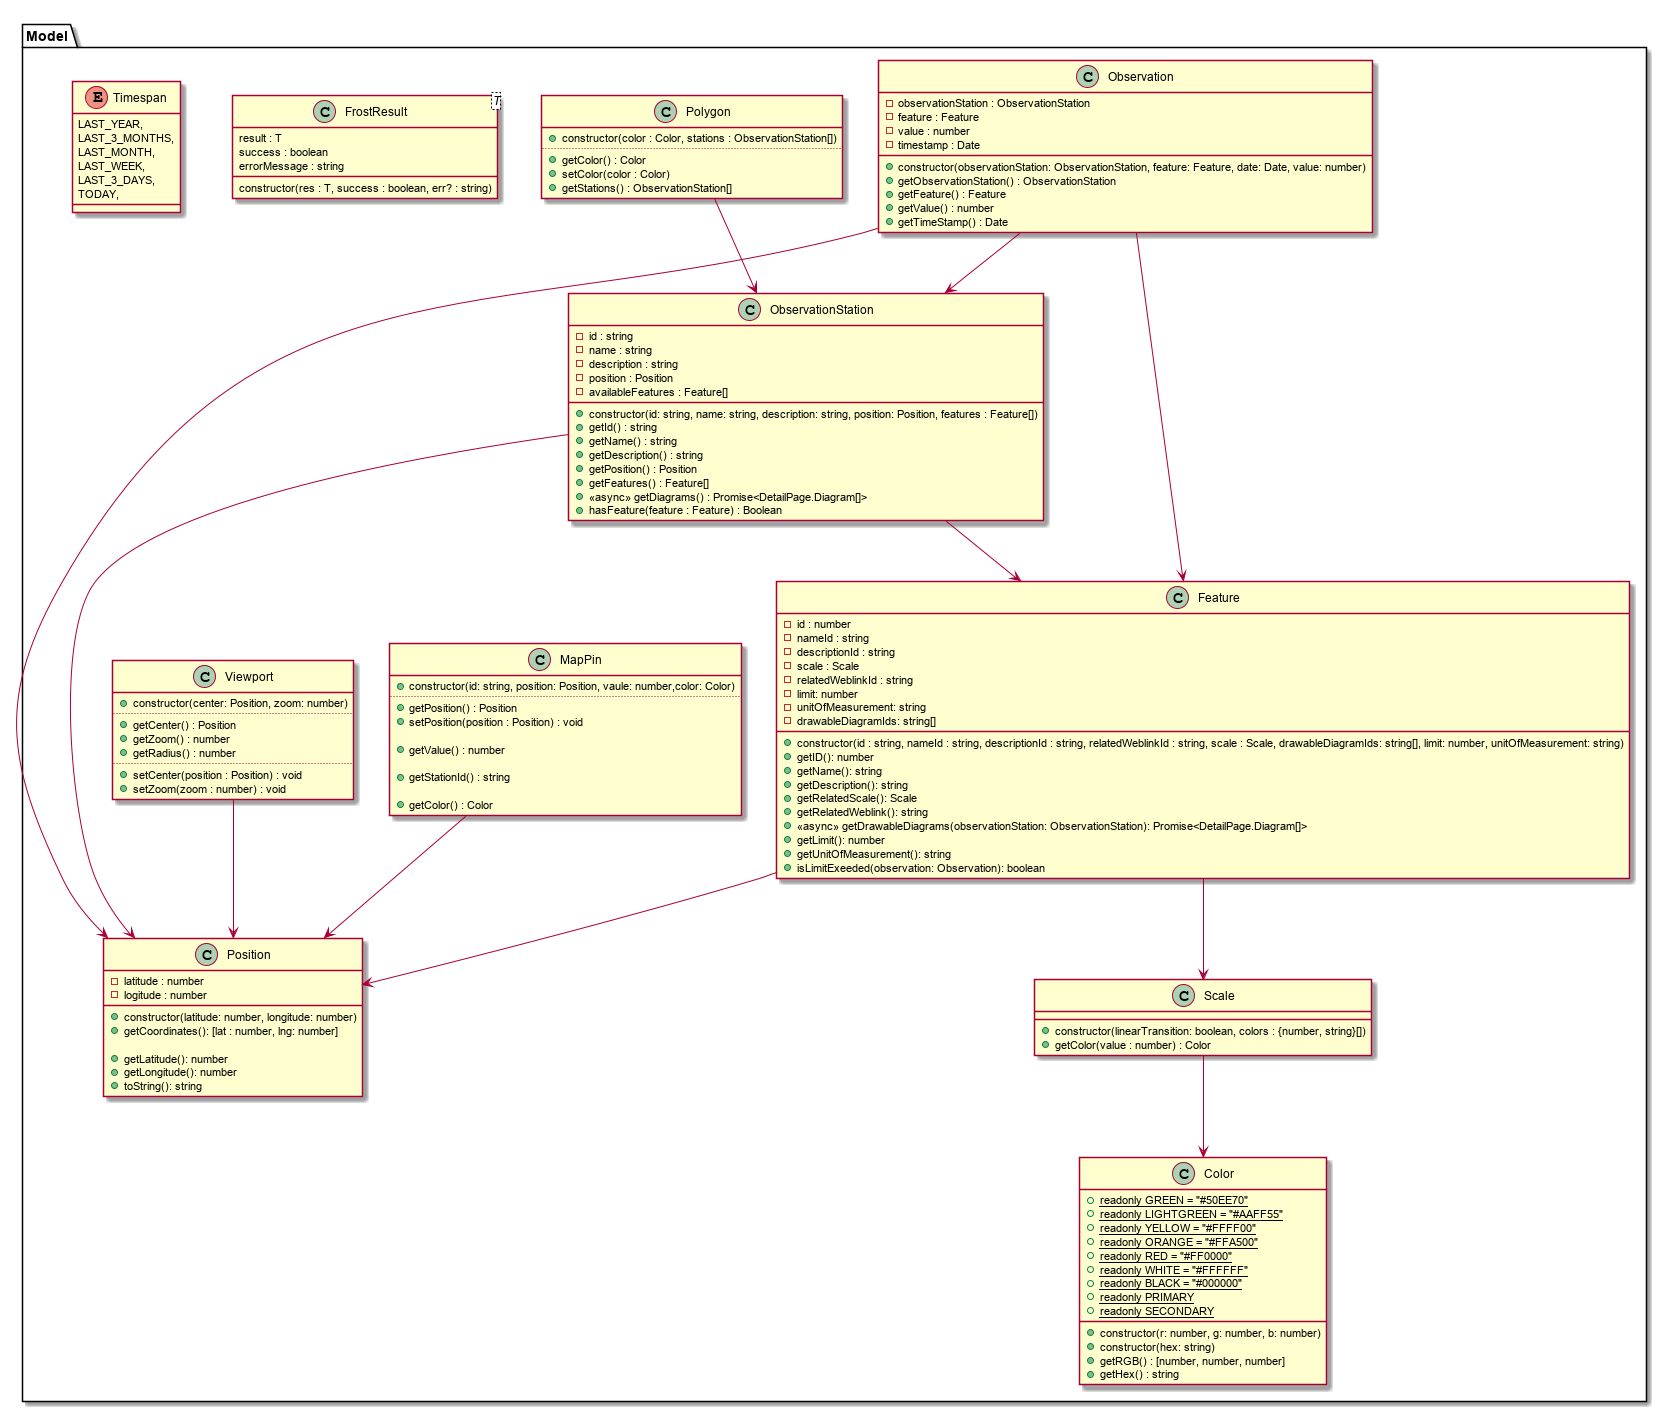
\includegraphics[angle=90, origin=c, height=\textwidth]{MVC/Model/Model.png}
\newpage

    \begin{Class}{FrostResult$\langle$T$\rangle$}
        FrostResult beinhaltet ein Objekt vom generischen Typ T und Metainformationen dazu.
        So können Fehler beim Erstellen des Objekts abgefangen und ggf. eine zweite Anfrage gestellt werden.
        \bigskip\\
        \textbf{Attribute}
        \begin{itemize}
            \item \texttt{result : T}
            \\ Falls \emph{success} true : Ein Objekt vom generischen Typ T
            \\ Falls \emph{success} false : nicht definiert.
            \item \texttt{success : boolean}
            \\ \emph{true} : Die Erzeugung von \emph{result} war erfolgreich.
            \\ \emph{false} : Erstellung von \emph{result} fehlgeschlagen.
            \item \texttt{errorMessage : string}
            \\ Nicht definiert wenn \emph{success} wahr ist.
            Sonst eine aussagekräftige Fehlermeldung über Probleme beim Erstellen von \emph{result}.
        \end{itemize}

        \textbf{Methoden}
        \begin{itemize}
            \item \texttt{constructor(result : T, success : boolean, err? : string)}
            \\ Wenn \emph{success} true : Setzt this.success auf true,  this.result auf result und this.errorMessage auf das leere Wort.
            \\ Sonst : Setzt this.result auf null, this.success auf false und this.errorMessage auf err.
        \end{itemize}
    \end{Class}

    \begin{Class}{ObservationStation}
        Eine Messstation mit Metadaten, verfügbaren Features und Diagrammen.
        \bigskip\\
        \textbf{Methoden}
        \begin{itemize}
            \item \texttt{constructor(id: string, name: string,
            \\ desc : string, pos: Position)}
            \\ Erstellt eine ObservationStation mit den angegebenen Attributen.
            Wirft einen Fehler wenn \emph{id} nicht das Format einer iot-id hat.
            \item \texttt{setFeatures(features : Features[])}
            \\ Setzt die unterstützten Features auf \emph{features}.
            \item \texttt{getId() : string}
            \\ Die iot-id der Station.
            \item \texttt{getName() : string}
            \\ Der Name der Station.
            \item \texttt{getDescription() : string}
            \\ Die Beschreibung der Station in der in \emph{Language} ausgewählten Sprache.
            \item \texttt{getFeatures() : Feature[]}
            \\ Array von Features, die die Station erfassen kann, und von der Anwendung unterstützt werden.
            \item \texttt{getPosition() : Position}
            \\ Die Position an der sich die Station befindet.
            \item \texttt{async getDiagrams() : Promise<DetailPage.Diagram[]>}
            \\ Liefert ein Promise auf ein Array an Diagrammen.
            Nach der Erfüllung werden die unterstützen Diagramme der verfügbaren Features ausgegeben.
            \item \texttt{hasFeature(feature : Feature) : boolean}
            \\ \emph{true} wenn die Station das Feature erfassen kann.
            \\ \emph{false} sonst.
        \end{itemize}
    \end{Class}

    \begin{Class}{Observation}
        Ein Messwert eines bestimmten Features an einer Messstation zu einem gewissen Zeitpunkt.
        \bigskip\\
        \textbf{Methoden}
        \begin{itemize}
            \item \texttt{constructor(observationStation: ObservationStation, 
            \\feature: Feature, date: Date, value: number)}
            \\ Erstellt eine Observation mit den angegebenen Attributen.
            \item \texttt{getObservationStation() : ObservationStation}
            \\ Die Messstation an der die Messung durchgeführt wurde.
            \item \texttt{getFeature() : Feature}
            \\ Gibt das Feature der Beobachtung zurück.
            \item \texttt{getTimeStamp() : Date}
            \\ Gibt den Zeitpunkt der Beobachtung zurück.
            \item \texttt{getValue() : number}
            \\ Gibt den Wert der Beobachtung (in der Einheit des Feature) zurück.
        \end{itemize}
    \end{Class}

    \begin{Class}{Position}
        Eine Position auf der Welt in Koordinaten.
        \bigskip\\
        \textbf{Methoden}
        \begin{itemize}
            \item \texttt{constructor(latitude: number, longitude: number)}
            \\ Erstellt eine Position an \emph{latitude} °N, \emph{longitude} °O
            \item \texttt{getCoordinates(): [number, number]}
            \\ Die Koordinaten der Position als [lat, lng] Tupel.
            \item \texttt{getLatitude(): number}
            \\ Die Latitude der Position.
            \item \texttt{getLongitude(): number}
            \\ Die Longitude der Position
            \item \texttt{toString() : string}
            \\ Gibt die Daten im Format 'N 0.00000°, O 0.00000°' als Zeichenkette zurück.
        \end{itemize}
    \end{Class}

    \begin{Class}{Feature}
        Eine Umwelteigenschaft die von einer Messstation gemessen werden kann, Metadaten
        und mögliche Diagramme.
        \bigskip\\
        \textbf{Methoden}
        \begin{itemize}
            \item \texttt{constructor(id : string, nameId : string, descriptionId : string,\\
             scale : Scale, relatedWeblinkId : string,
            \\drawableDiagramsId : string[],
            \\limit: number, unitOfMeasurement: string)}
            \\ Erstellt ein Feature mit den angegebenen Attributen.
            Wirft einen Fehler wenn \emph{scale} keine Farbstufen hat.
            \item \texttt{getId() : string}
            \\ Gibt die FROST-Id des Features zurück.
            \item \texttt{getName() : string}
            \\ Der lokalisierte Featurename in der aktuellen Sprache.
            \item \texttt{getUnitOfMeasurement() : string}
            \\ Gibt die Einheit in der das Feature angegeben ist zurück.
            \item \texttt{getDescription() : string}
            \\  Die lokalisierte Beschreibung in der aktuellen Sprache.
            \item \texttt{getRelatedScale() : Scale}
            \\ Die Farbskala des Features.
            \item \texttt{getRelatedWeblink(): string}
            \\ Eine URL zu einer Definition / Erklärung des gemessenen Wertes.
            \item \texttt{getLimit() : number}
            \\ Das Limit für eine Warnmeldung. Wenn das Limit -1 ist, wird nie eine Warnung ausgegeben.
            \item \texttt{isLimitExceeded(obs : Observation) : Boolean}
            \\ \emph{true} wenn der Wert der Observation das Limit des Features übersteigt.
            \\ \emph{false} wenn das Limit -1 ist oder der Wert der Observation <= Limit.
        \end{itemize}
    \end{Class}

    \begin{Class}{Color}
        Eine Klasse um Farben darzustellen und bequem zwischen RGB und Hex-Codierung umzuwandeln.
        \bigskip\\
        \textbf{Methoden}
        \begin{itemize}
            \item \texttt{constructor(r: number, g: number, b: number)}
            \\ Erstellt eine Farbe aus den RGB Werten.
            \item \texttt{constructor(hex: string)}
            \\ Erstellt eine Farbe aus dem Hexcode im Format '\#FFFFFF'.
            Entspricht \emph{hex} nicht dem Format wird ein Fehler geworfen.
            \item \texttt{getRGB() : [number, number, number]}
            \\ Die RGB Werte der Farbe als Zahlentripel.
            \item \texttt{getHex() : string}
            \\ Liefert den RGB-Wert der Farbe im Format '\#FFFFFF' zurück.
        \end{itemize}
    \end{Class}

    \begin{Class}{Scale}
        Skala, die einem Wert einen Farbenwert zuordnet. Mit dem Parameter "linearTransition" des Konstruktors kann eingestellt werden, ob es sich um eine diskrete, oder um eine stetige Skala handelt, bei der dann zwischen den vorgegebenen Farbwerten linear interpoliert wird.
        \bigskip\\
        \textbf{Methoden}
        \begin{itemize}
            \item \texttt{constructor(linearTransition: boolean,
            \\colors : {number, string}[])}
            \\ Erstellt eine Skala entsprechend der Attribute.
            Ist \emph{colors} leer wird ein Wert mit \{0, "\#BBBBBB"\} erstellt.
            \item \texttt{getColor(value : number) : Color}
            \\ Gibt die Farbe des Wertes entsprechend der Konfiguration zurück.
            Ist \emph{linearTransition} True wird die Farbe als Durchschnitt der zwei nächsten Farben berechnet.
        \end{itemize}
    \end{Class}

    \begin{Class}{Polygon}
        //Todo
        \bigskip\\
        \textbf{Methoden}
        \begin{itemize}
            \item \texttt{constructor(color : Color, stations : ObservationStation[])}
            \\ Erstellt ein Polygon mit den angegebenen Attributen.
            \item \texttt{getColor() : Color}
            \\ Die Farbe des Polygons
            \item \texttt{setColor(color : Color)}
            \\ Setzt die Farbe des Polygons auf \emph{color}
            \item \texttt{getStations() : ObservationStation[]}
            \\ Die Messstation die die Ecken des Polygons bilden.
        \end{itemize}
    \end{Class}

    \begin{Class}{MapPin}
        Ein Pin, der auf einer Karte eingezeichnet werden kann.
        \bigskip\\
        \textbf{Methoden}
        \begin{itemize}
            \item \texttt{constructor(id: string, position: Position, vaule: number,\\
            color: Color)}
            \\Constructor von Pin

            \bigskip
            \item \texttt{getPosition() : Position}
            \\ Liefert die Position des Pins
            \item \texttt{setPosition(position : Position) : void}
            \\ Setzt die Position des Pins
            \item \texttt{getValue() : number}
            \\ Liefert einen Wert zurück, der einem Pin zugewiesen werden kann.
            \item \texttt{getId() : string}
            \\ Liefert die Id des Pins.
            \item \texttt{getColor() : Color}
            \\ Liefert die Farbe des Pins.
        \end{itemize}
    \end{Class}

    \begin{Class}{Viewport}
        Ausschnitt einer Karte.
        \bigskip\\
        \textbf{Methoden}
        \begin{itemize}
            \item \texttt{constructor(center: Position, zoom: number)}
            \\ Konstruktor von Viewport
            \item \texttt{getCenter() : Position}
            \\ Liefert das Zentrum des Sichtfensters 
            \item \texttt{getZoom() : number}
            \\ Liefert das Zoomlevel des Sichtfensters
            \item \texttt{getRadius() : number}
            \\ Liefert den Durchmesser des Sichtfensters, 
            d.h. der Kreis um den Mittelpunkt der das ganze Sichtfenster einschließt.
            \item \texttt{setCenter(position : Position) : void}
            \\ Setzt das Zentrum des Fensters auf \emph{position}.
            \item \texttt{setZoom(zoom : number) : void}
            \\ Setzt das Zoomlevel auf \emph{zoom} wenn \emph{zoom} > 0.
        \end{itemize}
    \end{Class}

    \begin{Class}{<<enum>> Timespan}
        Timespan definiert einen Zeitabschnitt.
        \begin{itemize}
            \item \texttt{LAST\_YEAR}
            \item \texttt{LAST\_3\_MONTHS}
            \item \texttt{LAST\_MONTH}
            \item \texttt{LAST\_WEEK}
            \item \texttt{LAST\_3\_DAYS}
            \item \texttt{TODAY}
        \end{itemize}
    \end{Class}